%%%%%%%%%%%%%%%%%%%%%%
% This is an example presentation made with Christopher Gandrud's unofficial LSE Beamer theme
% Updated 27 December 2011
%%%%%%%%%%%%%%%%%%%%%%

\documentclass[xcolor={svgnames,usenames}]{beamer}
\usetheme{LSE}
\usepackage{color}
\usepackage{hyperref}
\hypersetup{colorlinks=true,linkcolor=black}
\usepackage{graphics}
\usepackage{pgf,tikz,pgfplots}
\usetikzlibrary{shapes,arrows,intersections,tikzmark}
\usetikzlibrary{matrix,fit,calc,trees,positioning,arrows,chains,shapes.geometric,shapes}
\usetikzlibrary{decorations.pathmorphing,patterns}
\usepackage{booktabs}
\usepackage{minted}
\usepackage{nicefrac}

% ----------------
% Disegni Tikz per differenze finite
% ----------------
\pgfdeclarelayer{edgelayer}
\pgfdeclarelayer{nodelayer}
\pgfsetlayers{edgelayer,nodelayer,main}

\tikzstyle{none}=[inner sep=0pt]

\usetikzlibrary{decorations.markings}
\usetikzlibrary{shapes.geometric}

\tikzstyle{rn}=[circle,fill=Red,draw=Black,line width=0.8 pt,inner sep=0p]
\tikzstyle{gn}=[circle,fill=Lime,draw=Black,line width=0.8 pt]
\tikzstyle{yn}=[circle,fill=Yellow,draw=Black,line width=0.8 pt]

\tikzstyle{simple}=[-,draw=Black,line width=2.000]
\tikzstyle{arrow}=[-,draw=Black,postaction={decorate},decoration={markings,mark=at position .5 with {\arrow{>}}},line width=2.000]
\tikzstyle{tick}=[-,draw=Black,postaction={decorate},decoration={markings,mark=at position .5 with {\draw (0,-0.1) -- (0,0.1);}},line width=2.000]

%%%%%%%%%%%%%%%%%%%%%%%%%%%%%%%% Title Slide %%%%%%%%%%%%%%%%%%%%%%%%%%
\title[Calcolo Parallelo]{Calcolo Parallelo : Lezione 2}
\author[F. Durastante]{
    \href{mailto:fabio.durastante@nunipi.it}{Fabio Durastante}
}
\institute{Dipartimento di Matematica, Università di Pisa}
\date[Maggio 2021]{Master in Scienze e Tecnologie Spaziali, 2022}

\beamerdefaultoverlayspecification{}

\begin{document}

\begin{frame}
	\titlepage
\end{frame}

\section[Outline]{}
\frame{\tableofcontents}

\section{A First Scientific Computation}

\begin{frame}[fragile]{The blocking send and receive}
\begin{minted}{c}
int MPI_Send(void *message, int count, 
MPI_Datatype datatype, int dest, int tag, 
MPI_Comm comm)
\end{minted}
\begin{description}
	\item[\textcolor{black}{\mintinline{c}{void *message}}] points to the message content itself, it can be a simple scalar or a group of data,
	\item[\textcolor{black}{\mintinline{c}{int count}}] specifies the number of data elements of which the message is composed,
	\item[\textcolor{black}{\mintinline{c}{MPI_Datatype datatype}}] indicates the \alert{data type} of the elements that make up the message,
	\item[\textcolor{black}{\mintinline{c}{int dest}}] the rank of the destination process, 
	\item[\textcolor{black}{\mintinline{c}{int tag}}] the user-defined tag field, 
	\item[\textcolor{black}{\mintinline{c}{MPI_Comm comm}}] the communicator in which the source and destination processes reside and for which their respective
	ranks are defined.
\end{description}
\end{frame}

\begin{frame}[fragile]{The blocking send and receive}
\begin{minted}{c}
int MPI_Recv (void *message, int count, 
MPI_Datatype datatype, int source, int tag,
MPI_Comm comm, MPI_Status *status)
\end{minted}
\begin{description}
\item[\textcolor{black}{\mintinline{c}{void *message}}] points to the message content itself, it can be a simple scalar or a group of data,
\item[\textcolor{black}{\mintinline{c}{int count}}] specifies the number of data elements of which the message is composed,
\item[\textcolor{black}{\mintinline{c}{MPI_Datatype datatype}}] indicates the \alert{data type} of the elements that make up the message,
\item[\textcolor{black}{\mintinline{c}{int source}}] the rank of the source process, 
\item[\textcolor{black}{\mintinline{c}{int tag}}] the user-defined tag field, 
\item[\textcolor{black}{\mintinline{c}{MPI_Comm comm}}] the communicator in which the source and destination processes reside,
\item[\textcolor{black}{\mintinline{c}{MPI_Status *status}}] is a structure that contains three fields named \mintinline{c}{MPI_SOURCE} , \mintinline{c}{MPI_TAG}, and \mintinline{c}{MPI_ERROR}.
\end{description}
\end{frame}

\begin{frame}[fragile]{Basic MPI Data Types}
Of the inputs in the previous slides the only one that is specific to MPI is the \mintinline{c}{MPI_Datatype}, these corresponds to a C data type
\begin{center}
	\begin{tabular}{ll}
		\toprule
		\mintinline{c}{MPI_CHAR} & \mintinline{c}{signed char} \\
		\mintinline{c}{MPI_SHORT} & \mintinline{c}{signed short int} \\
		\mintinline{c}{MPI_INT} & \mintinline{c}{signed int} \\
		\mintinline{c}{MPI_LONG} & \mintinline{c}{signed long int} \\
		\mintinline{c}{MPI_FLOAT} & \mintinline{c}{float} \\
		\mintinline{c}{MPI_DOUBLE} & \mintinline{c}{double} \\
		\mintinline{c}{MPI_LONG_DOUBLE} & \mintinline{c}{long double} \\
		\midrule
		\mintinline{c}{MPI_UNSIGNED_CHAR} & \mintinline{c}{unsigned char}\\
		\mintinline{c}{MPI_UNSIGNED_SHORT} & \mintinline{c}{unsigned short int}\\
		\mintinline{c}{MPI_UNSIGNED} & \mintinline{c}{unsigned int} \\
		\mintinline{c}{MPI_UNSIGNED_LONG} & \mintinline{c}{unsigned long int} \\
		\bottomrule
	\end{tabular}
\end{center}

\alert{Note}: we will see in the last lecture how to \mintinline{c}{send}/\mintinline{c}{receive} user--defined data structures.
\end{frame}

\begin{frame}{The 1\textsuperscript{st} derivative of a function with finite differences}
Given a function $f(x) : [a,b] \rightarrow \mathbb{R}$ we want to approximate $f'(x)$ on a (uniform) grid on the $[a,b]$ interval by using a finite difference scheme in parallel.

\begin{itemize}
	\item Given an integer $n \in \mathbb{N}$ we can subdivide the interval $[a,b]$ into intervals of length $\Delta x = \nicefrac{(b-a)}{n-1}$ with grid points $\{x_j\}_{j=0}^{n} = \{x_j = a + j \Delta x\}_{j=0}^{n-1}$:
	\begin{center}
		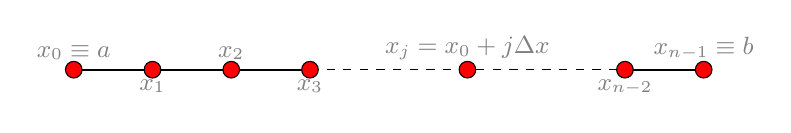
\begin{tikzpicture}
		\begin{pgfonlayer}{nodelayer}
		\node (0) at (0, -0) [circle,fill=Red,draw=Black,inner sep=0pt,minimum size=6pt]{};
		\node at (0,-0) [above]{\textcolor{gray}{\small $x_0 \equiv a$}};
		\node (0) at (1, -0) [circle,fill=Red,draw=Black,inner sep=0pt,minimum size=6pt]{};
		\node (1) at (1, -0) [below]{\textcolor{gray}{\small $x_1$}};
		\node (0) at (2, -0) [circle,fill=Red,draw=Black,inner sep=0pt,minimum size=6pt]{};
		\node (2) at (2, -0) [above]{\textcolor{gray}{\small $x_2$}};
		\node (0) at (3, -0) [circle,fill=Red,draw=Black,inner sep=0pt,minimum size=6pt]{};
		\node (3) at (3, -0) [below]{\textcolor{gray}{\small $x_3$}};
		\node (0) at (5, -0) [circle,fill=Red,draw=Black,inner sep=0pt,minimum size=6pt]{};
		\node (4) at (5, -0) [above]{\textcolor{gray}{\small $x_j = x_0 + j\Delta x$}};
		\node (0) at (7, -0) [circle,fill=Red,draw=Black,inner sep=0pt,minimum size=6pt]{};
		\node (5) at (7, -0) [below]{\textcolor{gray}{\small $x_{n-2}$}};
		\node (0) at (8, -0) [circle,fill=Red,draw=Black,inner sep=0pt,minimum size=6pt]{};
		\node (6) at (8, -0) [above]{\textcolor{gray}{\small $x_{n-1} \equiv b$}};
		\end{pgfonlayer}
		\begin{pgfonlayer}{edgelayer}
		\draw[thick] (0, -0) to (3, -0);
		\draw[dashed] (3, -0) to (7,-0);
		\draw[thick] (7, -0) to (8, -0);
		\end{pgfonlayer}
		\end{tikzpicture},
	\end{center}
	\item and consider the values $\{f_j\}_{j=0}^{n-1} = \{f(x_j)\}_{j=0}^{n-1}$
	\item We can approximate the values of $f'(x_j)$, for $j=1,\ldots,n-2$, by using only the values of $f$ at the knots $\{f_j\}_{j=0}^{n-1}$
\end{itemize}
\end{frame}
%
\begin{frame}{The 1\textsuperscript{st} derivative of a function with finite differences}
\begin{itemize}
\item<1-> The first derivative of $f$ at $x = x_j$ can be expressed by using knots for $j' > j$
\begin{equation*}
f'(x_j) \triangleq \lim_{\Delta x \rightarrow 0} \frac{f_{j+1} - f_j}{\Delta x} \approx \frac{f_{j+1} - f_j}{\Delta x} \triangleq D_+ f_j, \, 
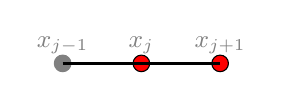
\begin{tikzpicture}
\node (0) at (0, -0) [circle,fill=gray,draw=gray,inner sep=0pt,minimum size=6pt]{};
\node at (0,-0) [above]{\textcolor{gray}{\small $x_{j-1}$}};
\node (0) at (1, -0) [circle,fill=Red,draw=Black,inner sep=0pt,minimum size=6pt]{};
\node (1) at (1, -0) [above]{\textcolor{gray}{\small $x_j$}};
\node (0) at (2, -0) [circle,fill=Red,draw=Black,inner sep=0pt,minimum size=6pt]{};
\node (2) at (2, -0) [above]{\textcolor{gray}{\small $x_{j+1}$}};
\draw[thick] (0, -0) to (2, -0);
\end{tikzpicture}
\end{equation*}
\item<2-> or equivalently by using knots for $j' < j$
\begin{equation*}
f'(x_j) \triangleq \lim_{\Delta x \rightarrow 0} \frac{f_{j} - f_{j-1}}{\Delta x} \approx \frac{f_{j} - f_{j-1}}{\Delta x} \triangleq D_- f_j, \, 
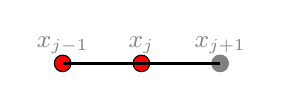
\begin{tikzpicture}
\node (0) at (0, -0) [circle,fill=Red,draw=Black,inner sep=0pt,minimum size=6pt]{};
\node at (0,-0) [above]{\textcolor{gray}{\small $x_{j-1}$}};
\node (0) at (1, -0) [circle,fill=Red,draw=Black,inner sep=0pt,minimum size=6pt]{};
\node (1) at (1, -0) [above]{\textcolor{gray}{\small $x_j$}};
\node (0) at (2, -0) [circle,fill=gray,draw=gray,inner sep=0pt,minimum size=6pt]{};
\node (2) at (2, -0) [above]{\textcolor{gray}{\small $x_{j+1}$}};
\draw[thick] (0, -0) to (2, -0);
\end{tikzpicture}
\end{equation*}	
\item<3-> at last we can consider the arithmetic mean of previous two:
\begin{equation*}
f'(x_j) \approx D_0 f_j \triangleq \frac{1}{2}(D_- f_j + D_+ f_j) = \frac{f_{j+1}-f_{j-1}}{2 \Delta x}, \, 
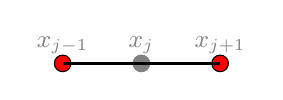
\begin{tikzpicture}
\node (0) at (0, -0) [circle,fill=Red,draw=Black,inner sep=0pt,minimum size=6pt]{};
\node at (0,-0) [above]{\textcolor{gray}{\small $x_{j-1}$}};
\node (0) at (1, -0) [circle,fill=gray,draw=gray,inner sep=0pt,minimum size=6pt]{};
\node (1) at (1, -0) [above]{\textcolor{gray}{\small $x_j$}};
\node (0) at (2, -0) [circle,fill=Red,draw=Black,inner sep=0pt,minimum size=6pt]{};
\node (2) at (2, -0) [above]{\textcolor{gray}{\small $x_{j+1}$}};
\draw[thick] (0, -0) to (2, -0);
\end{tikzpicture}
\end{equation*}
\end{itemize}
\end{frame}

\begin{frame}{Writing the sequential algorithm}
The sequential algorithms needs to break the approximation process into
three parts
\begin{enumerate}
\item evaluate the derivative $f'(x_i)$ for $i=1,\ldots,n-2$,
\item evaluate the derivative at the left--hand side $f'(x_0)$,
\item evaluate the derivative at the right--hand side $f'(x_{n-1})$.
\end{enumerate}
To have the same \emph{order of approximation} at each point of the grid we need to use a one--sided formula for the steps \alert{2.} and \alert{3.}, specifically
\begin{equation*}
f'(x_0) \approx \frac{-3 f_0 + 4 f_1 - f_2}{2 \Delta x}, \quad f'(x_{n-1}) \approx \frac{3f_{n-1} -4 f_{n-2} + f_{n-3}}{2 \Delta x}
\end{equation*}
\end{frame}

\begin{frame}[fragile]{Writing the sequential algorithm}
\small
Then the sequential algorithm can be written as
\begin{minted}{c}
void firstderiv1D_vec(int n, double dx, double *f, double *fx){
double scale;
scale = 1.0/(2.0*dx);
for (int i = 1; i < n-1; i++){
fx[i] = (f[i+1] - f[i-1])*scale;
}
fx[0] = (-3.0*f[0] + 4.0*f[1] - f[2])*scale;
fx[n-1] = (3.0*f[n-1] - 4.0*f[n-2] + f[n-3])*scale;
return;
}
\end{minted}
The function takes as input
\begin{itemize}
\item the number of grid points is $n$,
\item the amplitude of such intervals $\Delta x$,
\item the array containing the evaluation of $f$ (intent: input),
\item the array that will contain the value of the derivative (intent: output)
\end{itemize}
\end{frame}

\begin{frame}{Writing the parallel algorithm}
To implement the sequential differencing functions in parallel with MPI, we have to perform several steps
\begin{enumerate}
\item partition our domain $[a,b]$ among the processors,
\item each processor then computes the finite differences for all the points contained on that processor
\end{enumerate} 
\begin{onlyenv}<2>To actually perform the second step, we need to observe that the end-points on each subdomain needs information that is not contained on the processor, but that resides on a different one, we need to communicate boundary data!
\begin{center}
\definecolor{cccccc}{rgb}{0.8,0.8,0.8}
\definecolor{ffqqqq}{rgb}{1,0,0}
\begin{tikzpicture}[line cap=round,line join=round,>=triangle 45,x=0.8838091525664897cm,y=1.2369778701583198cm]
\clip(-3.26,-0.31) rectangle (10.32,1.31);
\draw (2,0)-- (5,0);
\draw (6,1)-- (9,1);
\draw (-2,1)-- (1,1);
\draw [dash pattern=on 1pt off 1pt] (1,1)-- (1,0);
\draw [dash pattern=on 1pt off 1pt] (2,1)-- (2,0);
\draw [dash pattern=on 1pt off 1pt] (5,1)-- (5,0);
\draw [dash pattern=on 1pt off 1pt] (6,1)-- (6,0);
\begin{scriptsize}
\fill [color=ffqqqq] (1,0) circle (2.0pt);
\fill [color=cccccc] (2,0) circle (2.0pt);
\fill [color=cccccc] (3,0) circle (2.0pt);
\fill [color=cccccc] (4,0) circle (2.0pt);
\fill [color=cccccc] (5,0) circle (2.0pt);
\fill [color=ffqqqq] (6,0) circle (2.0pt);
\fill [color=ffqqqq] (5,1) circle (2.0pt);
\fill [color=cccccc] (1,1) circle (2.0pt);
\fill [color=cccccc] (6,1) circle (2.0pt);
\fill [color=cccccc] (7,1) circle (2.0pt);
\fill [color=cccccc] (8,1) circle (2.0pt);
\fill [color=cccccc] (9,1) circle (2.0pt);
\fill [color=ffqqqq] (10,1) circle (2.0pt);
\fill [color=ffqqqq] (2,1) circle (2.0pt);
\fill [color=cccccc] (0,1) circle (2.0pt);
\fill [color=cccccc] (-1,1) circle (2.0pt);
\fill [color=cccccc] (-2,1) circle (2.0pt);
\fill [color=ffqqqq] (-3,1) circle (2.0pt);
\end{scriptsize}
\end{tikzpicture}
\end{center}
Red dots are \emph{halo} data, the one we need to communicate, while gray dots are data owned by the process. 
\end{onlyenv}
\end{frame}

\begin{frame}[fragile]{Writing the parallel algorithm}
The prototype of the function we want to write can be, in this case, 
\begin{minted}{c}
void firstderiv1Dp_vec(int n, double dx, double *f,
double *fx, int mynode, int totalnodes)
\end{minted}
where
\begin{itemize}
\item \mintinline{c}{int n} is the number of points per process,
\item \mintinline{c}{double dx} the amplitude of each interval,
\item \mintinline{c}{double *f, double *fx} the local portions with the values of $f(x)$ (input) and $f'(x)$ (output),
\item \mintinline{c}{int mynode} the rank of the current process,
\item \mintinline{c}{int totalnodes} the size of the communicator
\end{itemize}
We declare then the variables
\begin{minted}{c}
double scale = 1.0/(2.0*dx);
double mpitemp;
MPI_Status status;
\end{minted}
\end{frame}

\begin{frame}[fragile]{Writing the parallel algorithm}
Then we can treat the case in which we are at the beginning or at the end of the global interval
\begin{minted}{c}
if(mynode == 0){
fx[0] = (-3.0*f[0] + 4.0*f[1] - f[2])*scale;
}
if(mynode == (totalnodes-1)){
fx[n-1] = (3.0*f[n-1] - 4.0*f[n-2] + f[n-3])*scale;
}
\end{minted}
this approximate the derivative at the first and last point of the global interval. 
\vfill

\begin{onlyenv}<2>
Then, we can compute the inner part (the gray points) of the local interval by doing:
\begin{minted}{c}
for(int i=1;i<n-1;i++){
fx[i] = (f[i+1]-f[i-1])*scale;
}
\end{minted}
\end{onlyenv}
\end{frame}

\begin{frame}[fragile]{Writing the parallel algorithm}
The other case we need to treat is again the particular case in which we are in the first, or in the last interval. In both cases we have only one communication to perform
\begin{onlyenv}<1>
\begin{minted}{c}
if(mynode == 0){
mpitemp = f[n-1];
MPI_Send();
MPI_Recv();
fx[n-1] = (mpitemp - f[n-2])*scale;
}
else if(mynode == (totalnodes-1)){
MPI_Recv();
fx[0] = (f[1]-mpitemp)*scale;
mpitemp = f[0];
MPI_Send();
}
\end{minted}
\end{onlyenv}
\begin{onlyenv}<2>
\begin{minted}{c}
if(mynode == 0){
mpitemp = f[n-1];
MPI_Send(&mpitemp,1,MPI_DOUBLE,1,1,MPI_COMM_WORLD);
MPI_Recv(&mpitemp,1,MPI_DOUBLE,1,1,MPI_COMM_WORLD,&status);
fx[n-1] = (mpitemp - f[n-2])*scale;
}
else if(mynode == (totalnodes-1)){
MPI_Recv(&mpitemp,1,MPI_DOUBLE,mynode-1,1,MPI_COMM_WORLD, 
&status);
fx[0] = (f[1]-mpitemp)*scale;
mpitemp = f[0];
MPI_Send(&mpitemp,1,MPI_DOUBLE,mynode-1,1,MPI_COMM_WORLD);
}
\end{minted}
\end{onlyenv}
\end{frame}

\begin{frame}[fragile]{Writing the parallel algorithm}
Finally, the only remaining case is the one in which we need to communicate both the extremes of the interval
\begin{onlyenv}<1>
\begin{minted}{c}
else{
MPI_Recv();
fx[0] = (f[1]-mpitemp)*scale;
mpitemp = f[0];
MPI_Send();
mpitemp = f[n-1];
MPI_Send();
MPI_Recv();
fx[n-1] = (mpitemp-f[n-2])*scale;
}
\end{minted}
\end{onlyenv}
\begin{onlyenv}<2>
\begin{minted}{c}
else{
MPI_Recv(&mpitemp,1,MPI_DOUBLE,mynode-1,1,MPI_COMM_WORLD, 
&status);
fx[0] = (f[1]-mpitemp)*scale;
mpitemp = f[0];
MPI_Send(&mpitemp,1,MPI_DOUBLE,mynode-1,1,MPI_COMM_WORLD);
mpitemp = f[n-1];
MPI_Send(&mpitemp,1,MPI_DOUBLE,mynode+1,1,MPI_COMM_WORLD);
MPI_Recv(&mpitemp,1,MPI_DOUBLE,mynode+1,1,MPI_COMM_WORLD, 
&status);
fx[n-1] = (mpitemp-f[n-2])*scale;
}
\end{minted}
And the routine is complete!
\end{onlyenv}
\end{frame}

\begin{frame}[fragile]{Writing the parallel algorithm}
\footnotesize
A simple (and not very useful) principal program for this routine can be written by first initializing the parallel environment, and discovering who we are.
\begin{minted}{c}
MPI_Init( &argc, &argv );
MPI_Comm_rank( MPI_COMM_WORLD, &mynode );
MPI_Comm_size( MPI_COMM_WORLD, &totalnodes );
\end{minted}
Then we build the local values of the $f$ function
\begin{minted}{c}
globala = 0;
globalb = 1;
a = globala + ((double) mynode)*(globalb - globala)
/( (double) totalnodes);
b = globala + ((double) mynode+1)*(globalb - globala)
/( (double) totalnodes);
f  = (double *) malloc(sizeof(double)*(n));
fx = (double *) malloc(sizeof(double)*(n));
dx = (b-a)/((double) n);
for( int i = 0; i < n; i++){
f[i] = fun(a+((double) i)*dx);
}
\end{minted}
Finally we invoke our parallel computation
\mint{c}{firstderiv1Dp_vec( n, dx, f, fx, mynode, totalnodes);}
\end{frame}

\begin{frame}[fragile]{Writing the parallel algorithm}
To check if what we have done makes sens we evaluate the error in the $\|\cdot\|_2$ norm on the grid, i.e., $\sqrt{\Delta x} \| \mathbf{f}' - \mathbf{fx}\|_2$ on every process
\begin{minted}{c}
error = 0.0;
for(int i = 0; i < n; i++){
error += pow( fx[i]-funprime(a+((b-a)*((double) i))
/((double) n)),2.0);
}
error = sqrt(dx*error);
printf("Node %d ||f' - fx||_2 = %e\n",mynode,error);
\end{minted}
Then we clear the memory and close the parallel environment
\begin{minted}{c}
free(f);
free(fx);
MPI_Finalize();
\end{minted}
\end{frame}

%%%%%%%%%%%%%%%%%%%%%%%%%%%%%%%%%
\section{Collective Communications}

\begin{frame}{Collective Communications}
	A \alert{collective communication} is a communication that involves a group (or groups) of
	processes.
	\begin{itemize}
		\item the group of processes is represented as always as a \textcolor{blue}{communicator} that provides a context for the operation,
		\item Syntax and semantics of the collective
		operations are consistent with the syntax and semantics of the point-to-point
		operations,
		\item For collective operations, the amount of data sent \alert{must exactly match} the amount of data specified by
		the receiver.
	\end{itemize}
	\vfill
	\begin{block}<2>{Mixing type of calls}
	Collective communication calls may use the same communicators as point-to-point
	communication; Any (conforming) implementation of MPI messages guarantees that calls  generated on behalf of collective communication calls will not be confused with messages generated by point-to-point communication.
	\end{block}
\end{frame}

\subsection{Broadcast, Gather and Scatter}

\begin{frame}{Taxonomy of collective communications}

\begin{itemize}
	\item The \alert{broadcast} operation
\vfill
\begin{columns}
\begin{column}{0.5\columnwidth}
\centering
\tikzmark{x0} \qquad\qquad \tikzmark{x1}
\vspace{1em}

\begin{tabular}{c|c|c|c|c|}
	\cmidrule{2-5}
	\tikzmark{x2}\phantom{$a_0$}& $a_0$\tikzmark{a}   & \phantom{$a_0$} & \phantom{$a_0$}  & \phantom{$a_0$}  \\
	\cmidrule{2-5}
	& &    &    &    \\
	\cmidrule{2-5}
	& &    &    &    \\
	\cmidrule{2-5}
	\tikzmark{x3}\phantom{$a_0$}& &    &    &    \\
	\cmidrule{2-5}
\end{tabular}
\end{column}
\begin{column}{0.5\columnwidth}
\centering
\vspace{1em}

\begin{tabular}{c|c|c|c|c|}
	\cmidrule{2-5}
	& $a_0$\tikzmark{b}   & \phantom{$a_0$} & \phantom{$a_0$}  & \phantom{$a_0$}  \\
	\cmidrule{2-5}
	& $a_0$\tikzmark{c}&    &    &    \\
	\cmidrule{2-5}
	& $a_0$\tikzmark{d}&    &    &    \\
	\cmidrule{2-5}
	& $a_0$\tikzmark{e}&    &    &    \\
	\cmidrule{2-5}
\end{tabular}
\end{column}
\end{columns}

\begin{tikzpicture}[overlay,remember picture, shorten >=-4pt]
\draw[->,dashed] (pic cs:a) -- (pic cs:b);
\draw[->,dashed] (pic cs:a) -- (pic cs:c);
\draw[->,dashed] (pic cs:a) -- (pic cs:d);
\draw[->,dashed] (pic cs:a) -- (pic cs:e);
\draw[->,thick] (pic cs:x0) -- (pic cs:x1) node[above,midway] {data};
\draw[->,thick] (pic cs:x2) -- (pic cs:x3) node[midway,below,rotate=-90] {processes};
\end{tikzpicture}
In the broadcast, initially just the first process contains the data $a_0$, but after the broadcast all processes contain it.

\item This is an example of a \textbf{one-to-all} communication, i.e., only one process contributes to the result, while all processes receive the result.
\end{itemize}
\vfill
\end{frame}

\begin{frame}[fragile]{Taxonomy of collective communications: Broadcast}
\begin{minted}{c}
int MPI_Bcast(void* buffer, int count, 
 MPI_Datatype datatype, int root, MPI_Comm comm)
\end{minted}
Broadcasts a message from the process with rank \mintinline{c}{root} to all processes of the group, itself included.
\begin{description}
	\item[\textcolor{black}{\mintinline{c}{void* buffer}}] on return, the content of root's
	buffer is copied to all other processes.
	\item[\textcolor{black}{\mintinline{c}{int count}}] size of the message
	\item[\textcolor{black}{\mintinline{c}{MPI_Datatype datatype}}]  type of the \mintinline{c}{buffer}
	\item[\textcolor{black}{\mintinline{c}{int root}}] \mintinline{c}{rank} of the process broadcasting the message
	\item[\textcolor{black}{\mintinline{c}{MPI_Comm comm}}] communicator grouping the processes involved in the broadcast operation
\end{description}
\end{frame}

\begin{frame}{Taxonomy of collective communications: Scatter and Gather}

\begin{itemize}
	\item The \alert{scatter} and \alert{gather} operations
	\vfill
	\begin{columns}
		\begin{column}{0.5\columnwidth}
			\centering
			\tikzmark{x0} \qquad\qquad \tikzmark{x1}
			\vspace{0.35em}
			
			\begin{tabular}{c|c|c|c|c|}
				\cmidrule{2-5}
				\tikzmark{x2}\phantom{$a_0$}& $a_0$\tikzmark{a0}   & {$a_1$}\tikzmark{a1} & {$a_2$}\tikzmark{a2}  & {$a_3$}\tikzmark{a3}  \\
				\cmidrule{2-5}
				& &    &    &    \\
				\cmidrule{2-5}
				& &    &    &    \\
				\cmidrule{2-5}
				\tikzmark{x3}\phantom{$a_0$}& &    &    &    \\
				\cmidrule{2-5}
			\end{tabular}
		\end{column}
		\begin{column}{0.5\columnwidth}
			\centering
			\vspace{1em}
			
			\begin{tabular}{c|c|c|c|c|}
				\cmidrule{2-5}
				& $a_0$\tikzmark{b}   & \phantom{$a_0$} & \phantom{$a_0$}  & \phantom{$a_0$}  \\
				\cmidrule{2-5}
				& $a_1$\tikzmark{c}&    &    &    \\
				\cmidrule{2-5}
				& $a_2$\tikzmark{d}&    &    &    \\
				\cmidrule{2-5}
				& $a_3$\tikzmark{e}&    &    &    \\
				\cmidrule{2-5}
			\end{tabular}
		\end{column}
	\end{columns}
	
\begin{tikzpicture}[overlay,remember picture, shorten >=-4pt]
	\draw[<->,dashed] (pic cs:a0) -- (pic cs:b);
	\draw[<->,dashed] (pic cs:a1) -- (pic cs:c);
	\draw[<->,dashed] (pic cs:a2) -- (pic cs:d);
	\draw[<->,dashed] (pic cs:a3) -- (pic cs:e);
	\draw[->,thick] (pic cs:x0) -- (pic cs:x1) node[above,midway] {data};
	\draw[->,thick] (pic cs:x2) -- (pic cs:x3) node[midway,below,rotate=-90] {processes};
	\end{tikzpicture}
	\item In the \textbf{scatter}, initially just the first process contains the data $a_0,\ldots,a_3$, but after the \textbf{scatter} the $j$th process contains the $a_j$ data.
	\item In the \textbf{gather}, initially the $j$th process contains the $a_j$ data, but after the \textbf{gather} the first process contains the data $a_0,\ldots,a_3$
\end{itemize}
\vfill
\end{frame}

\begin{frame}[fragile]{Taxonomy of collective communications: Gather}
\small
Each process (root process included) sends the contents of its send buffer to the root process. The latter receives the messages and stores them in rank order.
\begin{minted}{c}
int MPI_Gather(const void* sendbuf, int sendcount, 
  MPI_Datatype sendtype,  void* recvbuf, int recvcount, 
  MPI_Datatype recvtype, int root, MPI_Comm comm)
\end{minted}
\begin{description}
\item[\textcolor{black}{\mintinline{c}{const void* sendbuf}}] starting address of send buffer
\item[\textcolor{black}{\mintinline{c}{int sendcount}}] number of elements in send buffer
\item[\textcolor{black}{\mintinline{c}{MPI_Datatype sendtype}}] data type of send buffer elements
\item[\textcolor{black}{\mintinline{c}{void* recvbuf}}] \alert<2>{address of receive buffer}
\item[\textcolor{black}{\mintinline{c}{int recvcount}}] \alert<2>{number of elements for any single receive} (and \underline{not} the total number of items!)
\item[\textcolor{black}{\mintinline{c}{MPI_Datatype recvtype}}] \alert<2>{data type of received buffer elements}
\item[\textcolor{black}{\mintinline{c}{int root}}] rank of receiving process
\item[\textcolor{black}{\mintinline{c}{MPI_Comm comm}}] communicator
\end{description}
\onslide<2>{\alert<2>{These are significant only at \mintinline{c}{root}!}}
\end{frame}

\begin{frame}[fragile]{Taxonomy of collective communications: Gather}
\small
Observe that
\begin{itemize}
	\item The type signature of \mintinline{c}{sendcount}, \mintinline{c}{sendtype} on each process must be equal to the type signature of \mintinline{c}{recvcount}, \mintinline{c}{recvtype} at all the processes. 
	\item The amount of data sent must be equal to the amount of data received, pairwise between each process and the root.
\end{itemize}
\begin{onlyenv}<2>
	Therefore, if we need to have a varying count of data from each process, we need to use instead 
\begin{minted}{c}
int MPI_Gatherv(const void* sendbuf, int sendcount, 
 MPI_Datatype sendtype, void* recvbuf, 
 const int recvcounts[], const int displs[], 
 MPI_Datatype recvtype, int root, MPI_Comm comm)
\end{minted}
	where
	\begin{description}
		\item[\textcolor{black}{\mintinline{c}{const int recvcounts[]}}] is an array (of length group size) containing the number of elements that are received from each process,
		\item[\textcolor{black}{\mintinline{c}{const int displs[]}}] is an array (of length group size). Entry \mintinline{c}{i} specifies
		the displacement relative to \mintinline{c}{recvbuf} at which to place the incoming data from process \mintinline{c}{i}.
	\end{description}
\end{onlyenv}
\end{frame}

\begin{frame}[fragile]{Taxonomy of collective communications: Gather}
\small
If we need to have the result of the \emph{gather} operation on every process involved in the communicator we can use the variant
\begin{minted}{c}
int MPI_Allgather(const void* sendbuf, int sendcount,
 MPI_Datatype sendtype, void* recvbuf, int recvcount,
 MPI_Datatype recvtype, MPI_Comm comm)
\end{minted}
\begin{itemize}
	\item All processes in the communicator \mintinline{c}{comm} receive the result. The block of data sent from the $j$th process is received
	by every process and placed in the $j$th block of the buffer \mintinline{c}{recvbuf}.
	\item The type signature associated with \mintinline{c}{sendcount}, \mintinline{c}{sendtype}, at a process must be equal to
	the type signature associated with \mintinline{c}{recvcount}, \mintinline{c}{recvtype} at any other process.
\end{itemize}
\begin{onlyenv}<2>
This function has also the version for gathering messages with different sizes:
\begin{minted}{c}
int MPI_Allgatherv(const void* sendbuf, int sendcount,
 MPI_Datatype sendtype, void* recvbuf, const int recvcounts[],
 const int displs[], MPI_Datatype recvtype, MPI_Comm comm)
\end{minted}
and works in a way analogous to the \mintinline{c}{MPI_Gatherv}.
\end{onlyenv}
\end{frame}


\begin{frame}[fragile]{Taxonomy of collective communications: Scatter}
This is simply the \emph{inverse} operation of \mintinline{c}{MPI_Gather}
\begin{minted}{c}
int MPI_Scatter(const void* sendbuf, int sendcount, 
  MPI_Datatype sendtype, void* recvbuf, int recvcount, 
  MPI_Datatype recvtype, int root, MPI_Comm comm)
\end{minted}
\begin{description}
\item[\textcolor{black}{\mintinline{c}{const void* sendbuf}}] \alert<2>{address of send buffer}
\item[\textcolor{black}{\mintinline{c}{int sendcount}}] \alert<2>{number of elements sent to each process}
\item[\textcolor{black}{\mintinline{c}{MPI_Datatype sendtype}}] \alert<2>{type of send buffer elements}
\item[\textcolor{black}{\mintinline{c}{void* recvbuf}}] address of receive buffer
\item[\textcolor{black}{\mintinline{c}{int recvcount}}] number of elements in receive buffer 
\item[\textcolor{black}{\mintinline{c}{MPI_Datatype recvtype}}] data type of receive buffer elements 
\item[\textcolor{black}{\mintinline{c}{int root}}]rank of sending process 
\item[\textcolor{black}{\mintinline{c}{MPI_Comm comm}}] communicator 
\end{description}
\onslide<2>{\alert{This choices are significant only at \mintinline{c}{root}!}}
\end{frame}

\begin{frame}[fragile]{Taxonomy of collective communications: Scatter}
\small
Observe that
\begin{itemize}
	\item The type signature of \mintinline{c}{sendcount}, \mintinline{c}{sendtype} on each process must be equal to the type signature of \mintinline{c}{recvcount}, \mintinline{c}{recvtype} at the root. 
	\item The amount of data sent must be equal to the amount of data received, pairwise between each process and the root.
\end{itemize}
\begin{onlyenv}<2>
	Therefore, if we need to have a varying count of data from each process, we need to use instead 
\begin{minted}{c}
int MPI_Scatterv(const void* sendbuf, const int sendcounts[],
 const int displs[], MPI_Datatype sendtype, void* recvbuf,
 int recvcount, MPI_Datatype recvtype, int root, MPI_Comm comm)
\end{minted}
	where
	\begin{description}
		\item[\textcolor{black}{\mintinline{c}{const int sendcounts[]}}] is an array (of length group size) containing the number of elements that are sent to each process,
		\item[\textcolor{black}{\mintinline{c}{const int displs[]}}] is an array (of length group size). Entry \mintinline{c}{i} specifies
		the displacement relative to \mintinline{c}{recvbuf} from which to take the outgoing data to process \mintinline{c}{i}.
	\end{description}
\end{onlyenv}
\end{frame}


\subsection{Modifying the 1\textsuperscript{st} derivative code}

\begin{frame}[fragile]{Modifying the 1\textsuperscript{st} derivative code}
	Let us perform the following modification to our first derivative code:
	\begin{enumerate}
		\item Taking from input the number of points to use in each interval,
		\item Collecting the whole result on one process and print it on file.
	\end{enumerate}
	\begin{onlyenv}
	For the first step we use the \mintinline{c}{MPI_Bcast} function,
	\begin{columns}
\begin{column}{0.5\columnwidth}
\begin{minted}{c}
if(mynode == 0){
 if(argc != 2){
  n = 20;
 }else{
  n = atoi(argv[1]);
 }
}
MPI_Bcast(&n,1,MPI_INT,
 0,MPI_COMM_WORLD);
\end{minted}
\end{column}
\begin{column}{0.5\columnwidth}
\begin{itemize}
	\item We read on \mintinline{c}{rank} $0$ the number \mintinline{c}{n} from command line,
	\item Then we broadcast it with \mintinline{c}{MPI_Bcast}, pay attention to the fact that the broadcast operations happens on all the processes!
\end{itemize}
\end{column}
	\end{columns}
	\end{onlyenv}
\end{frame}

\begin{frame}[fragile]{Modifying the 1\textsuperscript{st} derivative code}
Then we \emph{gather} all the derivatives from the various processes and collect them on process \mintinline{c}{0}.
\begin{columns}
	\begin{column}{0.5\columnwidth}
\begin{minted}{c}
if(mynode == 0)
 globalderiv = (double *) 
   malloc(sizeof(double) 
   *(n*totalnodes));

MPI_Gather(fx,n,MPI_DOUBLE,
  globalderiv,n,MPI_DOUBLE,
  0,MPI_COMM_WORLD);
\end{minted}
	\end{column}
\begin{column}{0.5\columnwidth}
\begin{itemize}
	\item we allocate on \mintinline{c}{rank 0} the memory that is necessary to store the whole derivative array,
	\item then we use the \mint{c}{MPI_Gather} to gather all the array \mintinline{c}{fx} (of \mintinline{c}{double}) inside
	the \mintinline{c}{globalderiv} array.
\end{itemize}
\end{column}
\end{columns}

At last we print it out on file on \mintinline{c}{rank 0}
\begin{minted}{c}
if(mynode == 0){
 FILE *fptr; fptr = fopen("derivative", "w");
 for(int i = 0; i < n*totalnodes; i++)
  fprintf(fptr,"%f %f\n",globala+i*dx,globalderiv[i]);
 fclose(fptr); free(globalderiv);}
\end{minted}
\end{frame}

\subsection{All-to-All Scatter/Gather}

\begin{frame}[fragile]{All-to-All}
\small
\mintinline{c}{MPI_ALLTOALL} is an extension of \mintinline{c}{MPI_ALLGATHER} to the case where each process
sends distinct data to each of the receivers.
\vspace{1em}
\begin{columns}
	\begin{column}{0.5\textwidth}
	\footnotesize
	\centering
	\tikzmark{all1} \qquad\qquad\qquad \tikzmark{all2}
	\vspace{1em}
	
	\begin{tabular}{c|c|c|c|c|}
		\cmidrule{2-5}
		\tikzmark{xx1}\phantom{$a_0$}&$a_0$ & $a_1$ & \ldots & $a_d$ \\
		\cmidrule{2-5}
		& $b_0$ & $b_1$ & \ldots & $c_d$ \\
		\cmidrule{2-5}
		& \vdots & \vdots & \ldots & \vdots \\
		\cmidrule{2-5}
		\tikzmark{xx2}\phantom{$a_0$}& $z_0$ & $z_1$ & \ldots & $z_d$ \\
		\cmidrule{2-5}
	\end{tabular}\hspace{1em}\tikzmark{group1}
	\end{column}
	\begin{column}{0.5\textwidth}
	\centering
	\footnotesize
	\tikzmark{all3} \qquad\qquad\qquad \tikzmark{all4}
	\vspace{1em}
	
	\tikzmark{group2}\hspace{1em}\begin{tabular}{|c|c|c|c|}
	\toprule
	$a_0$ & $b_0$ & \ldots & $z_1$ \\
	\midrule
	$a_1$ & $b_1$ & \ldots & $z_2$ \\
	\midrule
	\vdots & \vdots & \ldots & \vdots \\
	\midrule
	$a_d$ & $b_d$ & \ldots & $z_d$ \\
	\midrule
	\end{tabular}
	\end{column}
\end{columns}

\begin{tikzpicture}[overlay,remember picture, shorten >=-4pt]
\draw[->,thick] (pic cs:all1) -- (pic cs:all2) node[above,midway] {data};
\draw[->,thick] (pic cs:all3) -- (pic cs:all4) node[above,midway] {data};
\draw[->,thick] (pic cs:xx1) -- (pic cs:xx2) node[midway,below,rotate=-90] {processes};
\draw[->,thick] (pic cs:group1) -- (pic cs:group2);
\end{tikzpicture}
\vspace{0.5em}
\begin{minted}{c}
int MPI_Alltoall(const void* sendbuf, int sendcount,
 MPI_Datatype sendtype, void* recvbuf, int recvcount, 
 MPI_Datatype recvtype, MPI_Comm comm)
\end{minted}
\begin{itemize}
	\item The $j$th block sent from process $i$ is received by process $j$ and is placed in the $i$th block of \mintinline{c}{recvbuf}.
	\item The type signature for \mintinline{c}{sendcount}, \mintinline{c}{sendtype}, at a process must be equal to
	the type signature for \mintinline{c}{recvcount}, \mintinline{c}{recvtype} at any other process.
\end{itemize}
\end{frame}

\begin{frame}[fragile]{All-to-All different data size}
\small\vspace{-1em}
If we need to send data of different size between the processes
\begin{minted}{c}
int MPI_Alltoallv(const void* sendbuf, const int sendcounts[],
 const int sdispls[], MPI_Datatype sendtype, void* recvbuf,
 const int recvcounts[], const int rdispls[],
 MPI_Datatype recvtype, MPI_Comm comm);
\end{minted}
\vspace{-0.8em}
\begin{description}
\item[\textcolor{black}{\mintinline{c}{const void* sendbuf}}] starting address of send buffer
\item[\textcolor{black}{\mintinline{c}{const int sendcounts[]}}] array  specifying the number of elements to send to each rank
\item[\textcolor{black}{\mintinline{c}{const int sdispls[]}}] entry $j$ specifies
the displacement (relative to \mintinline{c}{sendbuf}) from which to
take the outgoing data destined for process $j$
\item[\textcolor{black}{\mintinline{c}{void* recvbuf}}] array specifying the number of elements that can be received from each rank
\item[\textcolor{black}{\mintinline{c}{const int recvcounts[]}}] integer array. Entry $i$ specifies
the displacement (relative to \mintinline{c}{recvbuf}) at which to place the incoming data from process $i$
\item[\textcolor{black}{\mintinline{c}{const int rdispls[]}}] entry $i$ specifies
the displacement (relative to \mintinline{c}{recvbuf}) at which to place
the incoming data from process $i$
\end{description}
\end{frame}

\subsection{Global reduce operation}

\begin{frame}[fragile]{The reduce operation}
The reduce operation for a given operator takes a data buffer from each of the processes in the communicator group and combines it according to operator rules.
\begin{minted}{c}
int MPI_Reduce(const void* sendbuf, void* recvbuf, 
 int count, MPI_Datatype datatype, MPI_Op op, 
 int root, MPI_Comm comm);
\end{minted}
\begin{description}
\item[\textcolor{black}{\mintinline{c}{const void* sendbuf}}] address of send buffer
\item[\textcolor{black}{\mintinline{c}{void* recvbuf}}] address of receive buffer
\item[\textcolor{black}{\mintinline{c}{int count}}] number of elements in send buffer
\item[\textcolor{black}{\mintinline{c}{MPI_Datatype datatype}}] data type of elements of send buffer
\item[\textcolor{black}{\mintinline{c}{MPI_Op op}}] reduce operation
\item[\textcolor{black}{\mintinline{c}{int root}}] rank of root process
\item[\textcolor{black}{\mintinline{c}{MPI_Comm comm}}] communicator
\end{description}
\end{frame}

\begin{frame}[fragile]{The reduce operation}
The value of \mintinline{c}{MPI_Op op} for the reduce operation can be taken from any of the following operators.

\begin{tabular}{ll|ll}
	\toprule
	\mintinline{c}{MPI_MAX} & Maximum & \mintinline{c}{MPI_MAXLOC} & Max value and location \\
	\mintinline{c}{MPI_MIN} & Minimum & \mintinline{c}{MPI_MINLOC} & Minimum value and location \\
	\mintinline{c}{MPI_SUM} & Sum & \mintinline{c}{MPI_LOR} & Logical or \\
	\mintinline{c}{MPI_PROD} & Product & \mintinline{c}{MPI_BOR} & Bit-wise or \\
	\mintinline{c}{MPI_LAND} & Logical and & \mintinline{c}{MPI_LXOR} & Logical exclusive or \\
	\mintinline{c}{MPI_BAND} & Bit-wise and & \mintinline{c}{MPI_BXOR} & Bit-wise exclusive or \\
	\bottomrule
\end{tabular}
\vfill
\begin{onlyenv}<2>
Moreover, if a different operator is needed, it is possible to create it by means of the function
\begin{minted}{c}
int MPI_Op_create(MPI_User_function* user_fn, int commute, 
MPI_Op* op)
\end{minted}

In C the prototype for a \mintinline{c}{MPI_User_function} is 
\begin{minted}{c}
typedef void MPI_User_function(void* invec, void* inoutvec, 
	int *len, MPI_Datatype *datatype);
\end{minted}
\end{onlyenv}
\end{frame}

\begin{frame}[fragile]{Global reduce operation -- All-Reduce}
\small
As for other collective operations we may want to have the result of the reduction available on every process in a group. 

The routine for obtaining such result is
\begin{minted}{c}
int MPI_Allreduce(const void* sendbuf, void* recvbuf, 
 int count, MPI_Datatype datatype, MPI_Op op, MPI_Comm comm)
\end{minted}
\begin{description}
	\item[\textcolor{black}{\mintinline{c}{const void* sendbuf}}] address of send buffer
	\item[\textcolor{black}{\mintinline{c}{void* recvbuf}}] address of receive buffer
	\item[\textcolor{black}{\mintinline{c}{int count}}] number of elements in send buffer
	\item[\textcolor{black}{\mintinline{c}{MPI_Datatype datatype}}] data type of elements of send buffer
	\item[\textcolor{black}{\mintinline{c}{MPI_Op op}}] reduce operation
	\item[\textcolor{black}{\mintinline{c}{MPI_Comm comm}}] communicator
\end{description}
This instruction behaves like a combination of a \emph{reduction} and \emph{broadcast} operation.
\end{frame}

\begin{frame}[fragile]{Global reduce operation -- All-Reduce-Scatter}
This is another variant of the reduction operation in which the result is \emph{scattered} to all processes in a group on return.
\begin{minted}{c}
int MPI_Reduce_scatter_block(const void* sendbuf, 
 void* recvbuf, int recvcount, MPI_Datatype datatype, 
 MPI_Op op, MPI_Comm comm);
\end{minted}
\begin{itemize}
\item The routine is called by all group members using the same arguments for \mintinline{c}{recvcount}, \mintinline{c}{datatype}, \mintinline{c}{op} and \mintinline{c}{comm}. 
\item The resulting vector is treated as \mintinline{c}{n} consecutive blocks of \mintinline{c}{recvcount} elements that are scattered to the processes of the group \mintinline{c}{comm}.
\item The $i$th block is sent to process $i$ and stored in the receive buffer defined by \mintinline{c}{recvbuf}, \mintinline{c}{recvcount}, and \mintinline{c}{datatype}.
\end{itemize}
\end{frame}

\begin{frame}[fragile]{Global reduce operation -- All-Reduce-Scatter}
Of this function also a variant with variable block--size is available
\begin{minted}{c}
int MPI_Reduce_scatter(const void* sendbuf, void* recvbuf,
const int recvcounts[], MPI_Datatype datatype, MPI_Op op,
MPI_Comm comm);
\end{minted}
\begin{itemize}
	\item This routine first performs a global element-wise reduction on vectors of $\verb|count|=\sum_{i=0}^{n-1}\verb|recevcounts[i]|$ elements in the send buffers defined by \mintinline{c}{sendbuf}, \mintinline{c}{count} and \mintinline{c}{datatype}, using the operation \mintinline{c}{op}, where \mintinline{c}{n} is the size of the communicator.
	\item The routine is called by all group members using the
	same arguments for \mintinline{c}{recvcounts}, \mintinline{c}{datatype}, \mintinline{c}{op} and \mintinline{c}{comm}.
	\item The resulting vector is treated as
	\mintinline{c}{n} consecutive blocks where the number of elements of the $i$th block is \mintinline{c}{recvcounts[i]}.
	\item The $i$th block is sent to process $i$ and
	stored in the receive buffer defined by \mintinline{c}{recvbuf}, \mintinline{c}{recvcounts[i]} and \mintinline{c}{datatype}.
\end{itemize}
\end{frame}

\section{Some computations using collective communications}

\subsection{Computing Integrals}
\begin{frame}{Computing integrals with parallel midpoint quadrature rule}
For an integrable function $f : [a,b] \rightarrow \mathbb{R}$ the \emph{midpoint} rule (sometimes \emph{rectangle} rule) is given by
\begin{equation*}
	\int_{a}^{b}f(x) dx \approx I_1 = (b-a) f\left(\frac{a+b}{2}\right),
\end{equation*}
\begin{columns}
\begin{column}{0.4\columnwidth}
This is a very crude approximation, to make it more accurate we may break up the interval $[a,b]$ into a number $n$ of non-overlapping subintervals $[a_k,b_k]$ such that $[a,b] = \cup_k [a_k,b_k]$,
\begin{equation*}
I_n =  \sum_{k=0}^n(b_k-a_k) f\left(\frac{a_k+b_k}{2}\right) 
\end{equation*}
\end{column}
\begin{column}{0.6\columnwidth}
\definecolor{wwffcc}{rgb}{0.4,1,0.8}
\definecolor{ffqqqq}{rgb}{1,0,0}
\definecolor{ffzzzz}{rgb}{1,0.6,0.6}
\definecolor{qqqqff}{rgb}{0,0,1}
\begin{tikzpicture}[line cap=round,line join=round,>=triangle 45,x=2.921158359000299cm,y=4.272671964665572cm]
\draw[->,color=black] (-0.03,0) -- (2.03,0);
\foreach \x in {,0.2,0.4,0.6,0.8,1,1.2,1.4,1.6,1.8,2}
\draw[shift={(\x,0)},color=black] (0pt,2pt) -- (0pt,-2pt) node[below] {\footnotesize $\x$};
\draw[->,color=black] (0,-0.05) -- (0,1.12);
\foreach \y in {,0.2,0.4,0.6,0.8,1}
\draw[shift={(0,\y)},color=black] (2pt,0pt) -- (-2pt,0pt) node[left] {\footnotesize $\y$};
\draw[color=black] (0pt,-10pt) node[right] {\footnotesize $0$};
\clip(-0.03,-0.05) rectangle (2.03,1.12);
\draw[line width=1.2pt,pattern color=ffzzzz,fill=ffzzzz,pattern=north east lines, smooth,samples=50,domain=0.0:2.0] plot(\x,{1/(1+\x^2)}) -- (2,0) -- (0,0) -- cycle;
\fill[color=wwffcc,fill=wwffcc,fill opacity=0.55] (0,0.99) -- (0.2,0.99) -- (0.2,0) -- (0,0) -- cycle;
\fill[color=wwffcc,fill=wwffcc,fill opacity=0.55] (0.2,0.92) -- (0.4,0.92) -- (0.4,0) -- (0.2,0) -- cycle;
\fill[color=wwffcc,fill=wwffcc,fill opacity=0.55] (0.4,0.8) -- (0.6,0.8) -- (0.6,0) -- (0.4,0) -- cycle;
\fill[color=wwffcc,fill=wwffcc,fill opacity=0.55] (0.6,0.67) -- (0.8,0.67) -- (0.8,0) -- (0.6,0) -- cycle;
\fill[color=wwffcc,fill=wwffcc,fill opacity=0.55] (0.8,0.55) -- (1,0.55) -- (1,0) -- (0.8,0) -- cycle;
\fill[color=wwffcc,fill=wwffcc,fill opacity=0.55] (1,0.45) -- (1.2,0.45) -- (1.2,0) -- (1,0) -- cycle;
\fill[color=wwffcc,fill=wwffcc,fill opacity=0.55] (1.2,0.37) -- (1.4,0.37) -- (1.4,0) -- (1.2,0) -- cycle;
\fill[color=wwffcc,fill=wwffcc,fill opacity=0.55] (1.4,0.31) -- (1.6,0.31) -- (1.6,0) -- (1.4,0) -- cycle;
\fill[color=wwffcc,fill=wwffcc,fill opacity=0.55] (1.6,0.26) -- (1.8,0.26) -- (1.8,0) -- (1.6,0) -- cycle;
\fill[color=wwffcc,fill=wwffcc,fill opacity=0.55] (1.8,0.22) -- (2,0.22) -- (2,0) -- (1.8,0) -- cycle;
\draw[line width=1.2pt, smooth,samples=100,domain=-0.02575841526514986:2.028221295048592] plot(\x,{1/(1+(\x)^2)});
\draw [color=wwffcc] (0,0.99)-- (0.2,0.99);
\draw [color=wwffcc] (0.2,0.99)-- (0.2,0);
\draw [color=wwffcc] (0.2,0)-- (0,0);
\draw [color=wwffcc] (0,0)-- (0,0.99);
\draw [color=wwffcc] (0.2,0.92)-- (0.4,0.92);
\draw [color=wwffcc] (0.4,0.92)-- (0.4,0);
\draw [color=wwffcc] (0.4,0)-- (0.2,0);
\draw [color=wwffcc] (0.2,0)-- (0.2,0.92);
\draw [color=wwffcc] (0.4,0.8)-- (0.6,0.8);
\draw [color=wwffcc] (0.6,0.8)-- (0.6,0);
\draw [color=wwffcc] (0.6,0)-- (0.4,0);
\draw [color=wwffcc] (0.4,0)-- (0.4,0.8);
\draw [color=wwffcc] (0.6,0.67)-- (0.8,0.67);
\draw [color=wwffcc] (0.8,0.67)-- (0.8,0);
\draw [color=wwffcc] (0.8,0)-- (0.6,0);
\draw [color=wwffcc] (0.6,0)-- (0.6,0.67);
\draw [color=wwffcc] (0.8,0.55)-- (1,0.55);
\draw [color=wwffcc] (1,0.55)-- (1,0);
\draw [color=wwffcc] (1,0)-- (0.8,0);
\draw [color=wwffcc] (0.8,0)-- (0.8,0.55);
\draw [color=wwffcc] (1,0.45)-- (1.2,0.45);
\draw [color=wwffcc] (1.2,0.45)-- (1.2,0);
\draw [color=wwffcc] (1.2,0)-- (1,0);
\draw [color=wwffcc] (1,0)-- (1,0.45);
\draw [color=wwffcc] (1.2,0.37)-- (1.4,0.37);
\draw [color=wwffcc] (1.4,0.37)-- (1.4,0);
\draw [color=wwffcc] (1.4,0)-- (1.2,0);
\draw [color=wwffcc] (1.2,0)-- (1.2,0.37);
\draw [color=wwffcc] (1.4,0.31)-- (1.6,0.31);
\draw [color=wwffcc] (1.6,0.31)-- (1.6,0);
\draw [color=wwffcc] (1.6,0)-- (1.4,0);
\draw [color=wwffcc] (1.4,0)-- (1.4,0.31);
\draw [color=wwffcc] (1.6,0.26)-- (1.8,0.26);
\draw [color=wwffcc] (1.8,0.26)-- (1.8,0);
\draw [color=wwffcc] (1.8,0)-- (1.6,0);
\draw [color=wwffcc] (1.6,0)-- (1.6,0.26);
\draw [color=wwffcc] (1.8,0.22)-- (2,0.22);
\draw [color=wwffcc] (2,0.22)-- (2,0);
\draw [color=wwffcc] (2,0)-- (1.8,0);
\draw [color=wwffcc] (1.8,0)-- (1.8,0.22);
\begin{scriptsize}
\fill [color=qqqqff] (0,0) circle (1.5pt);
\fill [color=qqqqff] (2,0) circle (1.5pt);
\fill [color=qqqqff] (0.2,0) circle (1.5pt);
\fill [color=qqqqff] (0.4,0) circle (1.5pt);
\fill [color=qqqqff] (0.6,0) circle (1.5pt);
\fill [color=qqqqff] (0.8,0) circle (1.5pt);
\fill [color=qqqqff] (1,0) circle (1.5pt);
\fill [color=qqqqff] (1.2,0) circle (1.5pt);
\fill [color=qqqqff] (1.4,0) circle (1.5pt);
\fill [color=qqqqff] (1.6,0) circle (1.5pt);
\fill [color=qqqqff] (1.8,0) circle (1.5pt);
\draw [color=ffqqqq] (0.1,0)-- ++(-2.0pt,-2.0pt) -- ++(4.0pt,4.0pt) ++(-4.0pt,0) -- ++(4.0pt,-4.0pt);
\draw [color=ffqqqq] (0.3,0)-- ++(-2.0pt,-2.0pt) -- ++(4.0pt,4.0pt) ++(-4.0pt,0) -- ++(4.0pt,-4.0pt);
\draw [color=ffqqqq] (0.5,0)-- ++(-2.0pt,-2.0pt) -- ++(4.0pt,4.0pt) ++(-4.0pt,0) -- ++(4.0pt,-4.0pt);
\draw [color=ffqqqq] (0.7,0)-- ++(-2.0pt,-2.0pt) -- ++(4.0pt,4.0pt) ++(-4.0pt,0) -- ++(4.0pt,-4.0pt);
\draw [color=ffqqqq] (0.9,0)-- ++(-2.0pt,-2.0pt) -- ++(4.0pt,4.0pt) ++(-4.0pt,0) -- ++(4.0pt,-4.0pt);
\draw [color=ffqqqq] (1.1,0)-- ++(-2.0pt,-2.0pt) -- ++(4.0pt,4.0pt) ++(-4.0pt,0) -- ++(4.0pt,-4.0pt);
\draw [color=ffqqqq] (1.3,0)-- ++(-2.0pt,-2.0pt) -- ++(4.0pt,4.0pt) ++(-4.0pt,0) -- ++(4.0pt,-4.0pt);
\draw [color=ffqqqq] (1.5,0)-- ++(-2.0pt,-2.0pt) -- ++(4.0pt,4.0pt) ++(-4.0pt,0) -- ++(4.0pt,-4.0pt);
\draw [color=ffqqqq] (1.7,0)-- ++(-2.0pt,-2.0pt) -- ++(4.0pt,4.0pt) ++(-4.0pt,0) -- ++(4.0pt,-4.0pt);
\draw [color=ffqqqq] (1.9,0)-- ++(-2.0pt,-2.0pt) -- ++(4.0pt,4.0pt) ++(-4.0pt,0) -- ++(4.0pt,-4.0pt);
\draw [color=ffqqqq] (0.1,0.99)-- ++(-2.0pt,-2.0pt) -- ++(4.0pt,4.0pt) ++(-4.0pt,0) -- ++(4.0pt,-4.0pt);
\draw [color=ffqqqq] (0.3,0.92)-- ++(-2.0pt,-2.0pt) -- ++(4.0pt,4.0pt) ++(-4.0pt,0) -- ++(4.0pt,-4.0pt);
\draw [color=ffqqqq] (0.5,0.8)-- ++(-2.0pt,-2.0pt) -- ++(4.0pt,4.0pt) ++(-4.0pt,0) -- ++(4.0pt,-4.0pt);
\draw [color=ffqqqq] (0.7,0.67)-- ++(-2.0pt,-2.0pt) -- ++(4.0pt,4.0pt) ++(-4.0pt,0) -- ++(4.0pt,-4.0pt);
\draw [color=ffqqqq] (0.9,0.55)-- ++(-2.0pt,-2.0pt) -- ++(4.0pt,4.0pt) ++(-4.0pt,0) -- ++(4.0pt,-4.0pt);
\draw [color=ffqqqq] (1.3,0.37)-- ++(-2.0pt,-2.0pt) -- ++(4.0pt,4.0pt) ++(-4.0pt,0) -- ++(4.0pt,-4.0pt);
\draw [color=ffqqqq] (1.5,0.31)-- ++(-2.0pt,-2.0pt) -- ++(4.0pt,4.0pt) ++(-4.0pt,0) -- ++(4.0pt,-4.0pt);
\draw [color=ffqqqq] (1.7,0.26)-- ++(-2.0pt,-2.0pt) -- ++(4.0pt,4.0pt) ++(-4.0pt,0) -- ++(4.0pt,-4.0pt);
\draw [color=ffqqqq] (1.9,0.22)-- ++(-2.0pt,-2.0pt) -- ++(4.0pt,4.0pt) ++(-4.0pt,0) -- ++(4.0pt,-4.0pt);
\draw [color=ffqqqq] (1.1,0.45)-- ++(-2.0pt,-2.0pt) -- ++(4.0pt,4.0pt) ++(-4.0pt,0) -- ++(4.0pt,-4.0pt);
\end{scriptsize}
\end{tikzpicture}
\end{column}
\end{columns}
\end{frame}

\begin{frame}{Computing integrals with parallel midpoint quadrature rule}
If we want to transform this computation in a parallel computation we can adopt the following sketch:
\begin{enumerate}
	\item \mintinline{c}{if (mynode == 0)} get number of intervals for quadrature
	\item broadcast number of intervals to all the processes
	\item assign the non-overlapping intervals to the processes
	\item sum function values in the center of each interval
	\item reduce with operator sum the integral on process 0.
\end{enumerate}
As a test function for the parallel integration routine we can use
\begin{equation*}
f(x) = \frac{4}{1+x^2}; \qquad I = \int_{0}^{1} \frac{4}{1+x^2} dx = \pi.
\end{equation*}
To evaluate the error we can use the value : \mintinline{c}{double PI25DT = 3.141592653589793238462643;}
\end{frame}

\begin{frame}[fragile]{Computing integrals with parallel midpoint quadrature rule}
\small
\begin{columns}
\begin{column}{0.4\columnwidth}
\begin{minted}{c}
h   = 1.0 / ((double) n*totalnodes);
sum = 0.0;
for (i = 1+mynode*n;
	i <= n*(mynode+1);
	i++){
 x = h * ((double)i - 0.5);
 sum += f(x);
}
mypi = h * sum;
MPI_Reduce(&mypi, &pi, 1, 
	MPI_DOUBLE, 
	MPI_SUM, 0, 
	MPI_COMM_WORLD);
\end{minted}
\end{column}
\begin{column}{0.6\columnwidth}
	\begin{itemize}
	\item We assume that all the intervals have the same size, thus the scaling \mintinline{c}{h   = 1.0 / (double) n},
	\item We compute all the value $x$ that are in the local process and increment the local sum,
	\item in conclusion we perform an \mintinline{c}{MPI_Reduce} to sum together all the local sums. 
	\end{itemize}
\end{column}
\end{columns}

\vfill
You can then print out the obtained value of $\pi$ and the error with respect to \mintinline{c}{PI25DT} as
\begin{minted}{c}
if (mynode == 0){
 printf("pi is approximately %.16f, Error is %e\n",
 	pi, fabs(pi - PI25DT));
}
\end{minted}
\end{frame}

\subsection{Random number generation: Montecarlo type algorithms}

\begin{frame}{Computing $\pi$ Montecarlo Style}
Montecarlo methods are algorithms that rely on a procedure of repeated random sampling to obtain numerical results\footnote{For some historical information about this idea: \url{https://bit.ly/3LKe38K}}.
\vfill

\begin{columns}
	\begin{column}{0.5\columnwidth}
	A generic Montecarlo algorithm can be described by the following 4 steps
		\begin{enumerate}
			\item define a domain of possible samples
			\item generate the samples from a probability distribution over such domain
			\item perform a deterministic computation on the inputs
			\item aggregate the results
		\end{enumerate}
	\end{column}
	\begin{column}{0.5\columnwidth}
	\onslide<2>{
	Let us use it to approximate $\pi$
	\begin{enumerate}
	\item we consider the square $S = [-1,1]\times[-1,1]$,
	\item we generate samples in $S$ from a uniform probability distribution
	\item we count the number of points $(x,y)$ that are such that $x^2 + y^2 \leq 1$,
	\item the approximation of $\pi$ is given by the ratio
	\[\pi \approx \nicefrac{ |\{(x,y) : \,x^2+y^2 \leq 1\}|}{|\{(x,y) \in S\}|} \]
	\end{enumerate}
	}
	\end{column}
	\end{columns}
\end{frame}

\begin{frame}{Computing $\pi$ Montecarlo Style}
We can write the parallel version of such algorithm in the following way
\vfill

\begin{columns}
	\begin{column}{0.5\columnwidth}
	\begin{enumerate}
	\item<2-> we divide a square in an number of parts equal to the number of processes we have,
	\item<3-> we generate a number of random points $(x,y)$ in the area owned by each process,
	\item<4-> we compute how many points fall in the circle
	\item<5-> sum-reduce the number of points in the square and in the circle
	\item<6-> divide the two numbers on process 0 to get the approximation
\end{enumerate}
	\end{column}
	\begin{column}{0.5\columnwidth}
\definecolor{fftttt}{rgb}{1,0.2,0.2}
\definecolor{ccccff}{rgb}{0.8,0.8,1}
\begin{tikzpicture}[line cap=round,line join=round,>=triangle 45,x=2.5cm,y=2.5cm]
\draw[->,color=black] (-1,0) -- (1,0);
\foreach \x in {-1}
\draw[shift={(\x,0)},color=black] (0pt,2pt) -- (0pt,-2pt) node[below] {\footnotesize $\x$};
\draw[->,color=black] (0,-1) -- (0,1);
\foreach \y in {-1}
\draw[shift={(0,\y)},color=black] (2pt,0pt) -- (-2pt,0pt) node[left] {\footnotesize $\y$};
\draw[color=black] (0pt,-10pt) node[right] {\footnotesize $0$};
\clip(-1,-1) rectangle (1,1);
\fill[color=ccccff,fill=ccccff,fill opacity=0.25] (-1,1) -- (1,1) -- (1,-1) -- (-1,-1) -- cycle;
\draw [color=fftttt,fill=fftttt,fill opacity=0.25] (0,0) circle (2.5cm);
\onslide<3->{\draw [color=ccccff] (-1,1)-- (1,1);
\draw [color=ccccff] (1,1)-- (1,-1);
\draw [color=ccccff] (1,-1)-- (-1,-1);
\draw [color=ccccff] (-1,-1)-- (-1,1);
\draw (-0.8,1)-- (-0.8,-1);
\draw (-0.6,-1)-- (-0.6,1);
\draw (-0.4,1)-- (-0.4,-1);
\draw (-0.2,-1)-- (-0.2,1);
\draw (0,1)-- (0,-1);
\draw (0.2,1)-- (0.2,-1);
\draw (0.4,-1)-- (0.4,1);
\draw (0.6,1)-- (0.6,-1);
\draw (0.8,-1)-- (0.8,1);
\draw (-1,0.8)-- (1,0.8);
\draw (-1,0.6)-- (1,0.6);
\draw (-1,0.4)-- (1,0.4);
\draw (-1,0.2)-- (1,0.2);
\draw (-1,0)-- (1,0);
\draw (-1,-0.2)-- (1,-0.2);
\draw (-1,-0.4)-- (1,-0.4);
\draw (-1,-0.6)-- (1,-0.6);
\draw (-1,-0.8)-- (1,-0.8);}
\end{tikzpicture}
	\end{column}
\end{columns}
\end{frame}

\begin{frame}[fragile]{A word of caution}
Generating random numbers in a meaningful way requires some care. This is true in general, but it is true in particular in a parallel environment. On each different process we need to be sure of generating \alert{independent sequences of random numbers}. This can be achieved by using different seeds for the random number generator.

We achieve this by using the \mintinline{c}{#include <time.h>} and \mintinline{c}{#include <rand.h>} libraries
\begin{minted}{c}
unsigned int seed = (unsigned) time(NULL);
\end{minted}
generates an integer on each process depending on the time of the call, then we build a seed by using \mintinline{c}{srand(seed + mynode)} that guarantees different seeds for the processes and thus independent random numbers:
\begin{minted}{c}
srand(seed + mynode);
x = rand_r(&seed); x = x / RAND_MAX; x = x1 + x * (x2 - x1);
y = rand_r(&seed); y = y / RAND_MAX; y = y1 + y * (y2 - y1);
\end{minted}
\end{frame}

\begin{frame}[fragile]{Computing $\pi$ Montecarlo Style}
We can generate on each node the sampling on the reference square by
\begin{minted}{c}
h  = 2.0 / (double) totalnodes;
x1 = -1.0 + mynode * h;
x2 = x1 + h;
y1 = -1.0;
y2 = 1.0;
my_SqPoints  = 0;
my_CiPoints  = 0;

for (i = 1; i <= n; i += totalnodes){
 srand(seed + mynode);
 x = rand_r(&seed); x = x / RAND_MAX; x = x1 + x * (x2 - x1);
 y = rand_r(&seed); y = y / RAND_MAX; y = y1 + y * (y2 - y1);
 my_SqPoints++;
 if ( ( x*x + y*y ) <= 1.0 ) my_CiPoints++;
}
\end{minted}
\end{frame}

\begin{frame}[fragile]{Computing $\pi$ Montecarlo Style}
\small
Then we perform the reduction by doing
\begin{minted}{c}
SqPoints = 0;
CiPoints = 0;
MPI_Reduce(&my_SqPoints, &SqPoints, 1, MPI_INT, MPI_SUM, 0,
 MPI_COMM_WORLD);
MPI_Reduce(&my_CiPoints, &CiPoints, 1, MPI_INT, MPI_SUM, 0,
 MPI_COMM_WORLD);
\end{minted}
and print the approximation
\begin{minted}{c}
if (mynode == 0){
pi = 4.0 * (double)CiPoints / (double)SqPoints;
printf("Pi is approximately %.16f, Error is %e\n"
 ,pi, fabs(pi - PI25DT));
}
\end{minted}
\end{frame}

\section{Timers and Synchronization}

\begin{frame}[fragile]{Timers and Synchronization}
\begin{itemize}
	\item<1-> A timer is specified even though it is not an instruction based on ``message-passing,'': timing parallel programs is important for inquiring on the ``performances'' of your code.
	\item<2-> the timer returns a floating-point number of seconds, representing elapsed wall-clock time since \emph{some time in the past}:
	\begin{minted}{c}
	double MPI_Wtime(void);
	\end{minted}
	the \emph{time in the past} is guaranteed not to change during the life of the process.
	\item<3-> the usual application of a timer is something of the form:
\begin{minted}{c}
double starttime, endtime;
starttime = MPI_Wtime();
< --- foolish things happen here --- >
endtime = MPI_Wtime();
printf("That took %f seconds\n",endtime-starttime);
\end{minted}
	\item<4-> There exists a tag \mintinline{c}{MPI_WTIME_IS_GLOBAL} that is 1 if clocks at all processes in \mintinline{c}{MPI_COMM_WORLD} are synchronized, 0 otherwise.
\end{itemize}
\end{frame}

\begin{frame}[fragile]{Timers and Synchronization}
\begin{itemize}
\item MPI offers a \emph{barrier} function that blocks the caller until all processes in the communicator have called it 
\mint{c}{int MPI_Barrier(MPI_Comm comm)}
that is, the call returns at any process only after all members of the communicator have entered the call. 
\item<2-> It can be used together with the \mintinline{c}{MPI_Wait} function to force a synchronization point in the program.
\item<3-> It can be used to regulate the access to an external resource (e.g., a file) in such a way that every processor accesses it in an order way: if you are interested in writing file in parallel you can look at Chapter 13 of the MPI guide\footnote<3->{Message Passing Interface Forum. MPI: A Message-Passing Interface Standard, Version 3.1. \url{https://www.mpi-forum.org/docs/mpi-3.1/mpi31-report.pdf}, High Performance Computing Center Stuttgart (HLRS).}
\end{itemize}

\end{frame}

\begin{frame}{Evaluating performances}
You can use the \mintinline{c}{MPI_Wtime()} to give a simple \alert{evalaution of the performances} of your program.
\medskip

Consider, e.g., the two programs for the computation of the $\pi$ constant. You can evaluate the \alert{weak scalability} of your code by looking at the time spent in doing the whole computation for growing size of processor numbers and samples. 
\medskip

We can compute the \alert{efficiency} of the code by measuring:
\begin{equation*}
	E = t(1)/t(N) \in [0,1]
\end{equation*}
where
\begin{itemize}
	\item $t(1)$ is the amount of time to complete a work unit with 1 processing element,
	\item $t(N)$ is the amount of time to complete N of the same work units with N processing elements.
\end{itemize}
\end{frame}

\begin{frame}{Further modifications}
For the derivative program:
\begin{itemize}
\item In every case the function \mintinline{c}{void firstderiv1Dp_vec} wants to exchange
information between two adjacent processes, i.e., every process wants to ``swap'' is halo with its adjacent process. We can rewrite the whole function by using the \mintinline{c}{MPI_Sendrecv_replace} point-to-point communication routine.
\item We can rewrite the entire program in an ``embarrassing parallel'' way, if every process has access to $f$, and are assuming that all the interval are partitioned the same way, by using the knowledge of our \mintinline{c}{rank} we can compute what are the boundary elements at the previous and following process. Thus, no communication at all!
\end{itemize}
For the $\pi$ programs, 
\begin{itemize}
	\item Make a graph of the timings to evaluate the \alert{weak scaling} efficiency.
\end{itemize}
\vfill
\begin{center} 
-- Try this at home! (Maybe here, if there is still time\ldots) --
\end{center}
\end{frame}

\end{document}